\chapter{Formulating Language Models as Weighted Sums}
\label{ch:weightedsum}

In this chapter we will present a novel way to represent the probabilities
$\ProbMKN{w_n}{w_1^{n-1}}$ and $\ProbGLM{w_n}{w_1^{n-1}}$ as weighted sums of
terms depending on $w_n$, for a fixed history $h = w_1^{n-1}$ and an  arbitrary
probability event $w = w_n$.
In other words we will express the formulas given in \cref{ch:review} as
equations of the following form:
\begin{equation}
  \label{eq:weightedsum}
  \Prob{w}{h} = \sum_{i = 1}^{N} \SumWeight_i^h \cdot \SumArg_i^h(w)
\end{equation}
Where $N$ is the number of interpolation factors dependent on the choice of
language model.

To the author's knowledge, there is no other work on expressing existing
language models as weighted sums.
However, \textcite{JelinekMercer1980} already experimented with learning
weighted sum parameters automatically for language modeling.

Being able to accurately represent probabilities in a form like this is highly
beneficial for word prediction.
As we can see in \cref{eq:prefixquery} the computation for next word prediction
is based on calculating multiple probabilities $\Prob{w}{h}$ with a fixed
history $h$ but varying arguments $w$.
As has been specified in \cref{ch:review}, probability calculation is based on
complex recursive formulas.
Using our weighted sum representation this computation can be sped up by
a huge factor, since the computation of the sum weights $\SumWeight^h_i$ can
be performed once beforehand.
For each final probability we then only have to perform the $N$ remaining
lookups $\SumArg^h_i(w)$ that actually depend on $w$.

Another handy benefit is that by this representation we have all terms that
change with $w$ explicitly available, which is a prerequisite for top-$k$
joining and will be explained in \cref{ch:topkjoin}.
Last, our algorithms for calculating sum weights turn out to be performing
faster than the direct recursive implementations, which we measure in
\cref{sec:evaluation-weightedsum}.

We will now present the basic idea of how to transform a probability
$\Prob{w_n}{w_1^{n-1}}$ into a weighted sum that applies to both Modified
Kneser-Ney Smoothing and the Generalized Language Model:

Note that in all \cref{eq:mkn-high,eq:mkn-low,eq:glm-high,eq:glm-low} the
probability event $w_n$ only appears in the nominator of fractions, specifically
in the argument terms of $\DiscountedCount$ or $\DiscountedCount*$.
Additionally $w_n$ occurs as arguments for $\Count$ and $\ContCountIp$ in the
lowest order \cref{eq:mkn-lowest,eq:glm-lowest}.
Our general idea is thus, to first expand recursive calls to
$\Prob(\DummyArg)$ or $\Prob*(\DummyArg)$, and second to factor
out the terms that do not depend on $w_n$ by the distributive property.

\Cref{sec:weightedsum-mkn} explains our approach for Modified Kneser-Ney
Smoothing, while \cref{sec:weightedsum-glm} concerns itself with the Generalized
Language Model.


% ------------------------------------------------------------------------------
\clearpage
\section{Modified Kneser-Ney Smoothing}
\label{sec:weightedsum-mkn}

Modified Kneser-Ney Smoothed probabilities $\ProbMKN{w}{h}$ are calculated as
follows (\cref{sec:review-lm-mkn}):
\begin{enumerate}
  \item Backing-off: Leave out words at the beginning of the history $h$, until
    $h \Skp$ is seen for the first time (\cref{eq:mkn-backoff}).
  \item Highest order: Look up frequency counts $\DiscountedCount(h \: w)$ and
    $\Count(h \Skp)$ (\cref{eq:mkn-high}) and shorten the history by one word.
  \item Lower orders: Look up continuation counts $\DiscountedCount*(\WSkp h \: w)$
    and $\ContCountIp(\WSkp h \WSkp)$ (\cref{eq:mkn-low}) and shorten the
    history further until it is empty.
  \item Lowest order: Look up continuation counts $\ContCountIp(\WSkp w)$ and
    $\ContCountIp(\WSkp \WSkp)$ (\cref{eq:mkn-lowest}).
\end{enumerate}

\newcommand{\ProbMKNcab}[1]
  {\frac{\DiscountedCount(w_1 w_2 w_3) + \gamma(w_1 w_2) #1}{\Count(w_1 w_2 \Skp)}}
\newcommand{\ProbMKNcb}[1]
  {\frac{\DiscountedCount*(\WSkp w_2 w_3) + \gamma(w_2) #1}{\ContCountIp(\WSkp w_2 \WSkp)}}
\newcommand{\ProbMKNc}
  {\frac{\ContCountIp(\WSkp w_3)}{\ContCountIp(\WSkp \WSkp)}}

% - - - - - - - - - - - - - - - - - - - - - - - - - - - - - - - - - - - - - - -
\subsection{Example}

As an example we will give the full formula expansion necessary to calculate
$\ProbMKN{w_3}{w_1 w_2}$ for any sequence $w_1 w_2 w_3$, assuming sequence
$w_1 w_2 \Skp$ was seen:
\begin{subequations}
  \begin{align}
    \ProbMKN {w_3}{w_1 w_2} &= \ProbMKNcab{\ProbMKN*{w_3}{w_2}} \\
    \ProbMKN*{w_3}{w_2}     &= \ProbMKNcb{\ProbMKN*{w_3}} \\
    \ProbMKN*{w_3}          &= \ProbMKNc
  \end{align}
\end{subequations}
Inserting the lower orders results in:
\begin{equation}
  \ProbMKN {w_3}{w_1 w_2} = \ProbMKNcab{\ProbMKNcb{\ProbMKNc}}
\end{equation}
By using the distributive property we obtain:
\begin{align}
  \label{eq:probmknexpansion-final}
  \hspace{-2.5em}\ProbMKN {w_3}{w_1 w_2} = {}
    & & \DiscountedCount (w_1 w_2 w_3)   & \cdot\ \frac{1}{\Count(w_1 w_2 \Skp)} \\
    &+& \DiscountedCount*(\WSkp w_2 w_3) & \cdot\ \frac{\gamma(w_1 w_2)}{\Count(w_1 w_2 \Skp) \ContCountIp(\WSkp w_2 \WSkp)} \nonumber \\
    &+& \ContCountIp(\WSkp w_3)          & \cdot\ \frac{\gamma(w_1 w_2) \: \gamma(w_2)}{\Count(w_1 w_2 \Skp) \ContCountIp(\WSkp w_2 \WSkp) \ContCountIp(\WSkp \WSkp)} \nonumber
\end{align}

In the final equation \cref{eq:probmknexpansion-final} we can clearly identify
the terms that do depend on $w_3$ and the ones that do not.
Note that $w_3$ never occurs on the right side of the multiplication dot.
Per line the left side of the multiplication dot will form the terms
$\SumArg^h_i(w_3)$, while the right side will form the sum weights
$\SumWeight^h_i$.

But note that this is only valid if the sequence $w_1 w_2 w_3$ has been seen in
the training corpus, and thus $\Count(w_1 w_2 w_3) \geq 1$.
If this is not the case, backoff steps have to be performed, and a different
resulting formula is obtained.

% - - - - - - - - - - - - - - - - - - - - - - - - - - - - - - - - - - - - - - -
\subsection{Sum Terms}

All counts except the ones of the lowest order are discounted using
$\DiscountedCount$ and $\DiscountedCount*$ to interpolate that order with the
following by the weight $\gamma(h)$.
This process of interpolating different orders is visualized in
\cref{fig:history-mkn} for the case of a history of length three.
Building similar backoff graphs for other history lengths is straightforward.

\begin{figure}[tb]
  \centering
  \documentclass{standalone}
\usepackage[dvipsnames,svgnames,x11names]{xcolor}
\usepackage{tikz}
\usepackage{../thesismath}
\begin{document}
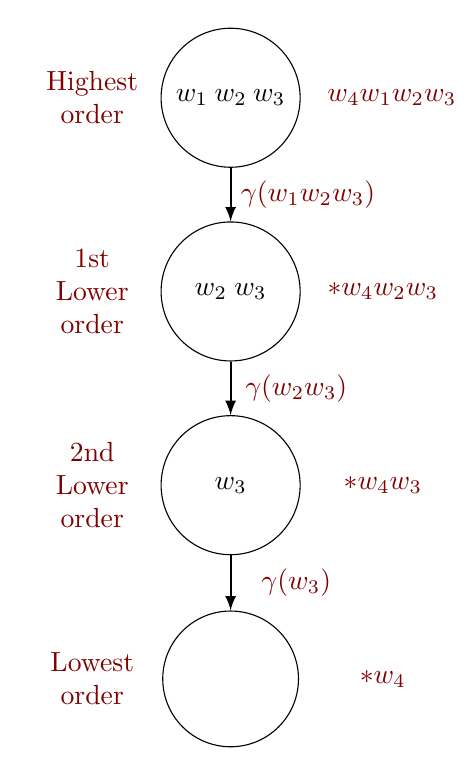
\begin{tikzpicture}
  \tikzset{
    state/.style  = {draw, circle, align = center, text centered, text width = 4.2em},
    invis/.style  = {text width = 4.2em},
    order/.style  = {align = center, text centered, text width = 4em, text = Maroon},
    number/.style = {xshift = 1em, text = Maroon},
  }

  \begin{scope}[node distance = 7em]
    \node [state] (highest)                    {$w_1 \: w_2 \: w_3$};
    \node [state] (lower1)  [below of=highest] {$w_2 \: w_3$};
    \node [state] (lower2)  [below of=lower1]  {$w_3$};
    \node [state] (lowest)  [below of=lower2]  {$\varnothing$};
  \end{scope}

  \begin{scope}[node distance = 5.5em]
    \node [order] [right of=highest] {$\ProbMKN {w_4}{w_1 w_2 w_3}$};
    \node [order] [right of=lower1]  {$\ProbMKN*{w_4}{w_2 w_3}$};
    \node [order] [right of=lower2]  {$\ProbMKN*{w_4}{w_3}$};
    \node [order] [right of=lowest]  {$\ProbMKN*{w_4}$};
  \end{scope}

  \begin{scope}[node distance = 5em]
    \node [order] [left of=highest] {Highest order};
    \node [order] [left of=lower1]  {1st Lower order};
    \node [order] [left of=lower2]  {2nd Lower order};
    \node [order] [left of=lowest]  {Lowest order};
  \end{scope}

  \path[->, >=latex, thick]
    (highest) edge node [right, order] {$\textstyle{\gamma(w_1 w_2 w_3)}$} (lower1)
    (lower1)  edge node [right, order] {$\textstyle{\gamma(w_2 w_3)}$}     (lower2)
    (lower2)  edge node [right, order] {$\textstyle{\gamma(w_3)}$}         (lowest);
\end{tikzpicture}
\end{document}

  \caption{
    The \emph{backoff graphs} shows the interpolation of different orders during
    computation of $\ProbMKN{w_4}{w_1 w_2 w_3}$.
    Centered are the histories for each probability.
    It is assumed that the history $w_1 w_2 w_3$ was seen during training, so
    that no backing-off is necessary.
    Orders are combined with interpolation weights $\gamma(\DummyArg)$.
  }
  \label{fig:history-mkn}
\end{figure}

Each order with a history $h^\prime$ is interpolated with the following order where
the first word of $h^\prime$ is removed.
Thus a total ordering on the histories of the orders can be specified.
In \cref{fig:history-mkn} we have thus assigned each history a number from
$1$~to~$4$.
Let $\DerivedHistory[i]$ denote the history of that graph with number $i$.

The first step in expressing $\ProbMKN{w}{h}$ as a weighted sum is finding the
number $N$ of sum weights.
In the case of Modified Kneser-Ney Smoothing this is exactly the number of
interpolation orders.
Let $\DerivedHistory[s]$ be the first seen history that is the result of
backing-off given history $h$ exactly $s$ times.
The number $N$ of sum weights is then the number of words of that history plus
one for the empty history.
\begin{equation}
  \label{eq:weightedsum-mkn-num}
  N = \NGramLength{\DerivedHistory[s]} + 1
\end{equation}
Where $\NGramLength{w_1^n} = n$ is the length of the $n$-gram $w_1^n$.

The next step is to find the actual terms $\SumArg_i^h(w)$ that shall be
weighted and added.
When looking at the equations that define Modified Kneser-Ney we note the fact
that only the count terms in the numerators depend on the probability event $w$.
Exactly these terms compose our sum arguments:
\begin{equation}
  \SumArg_i^h(w) =
    \begin{dcases*}
      \Count(w)                                             & if $N = 1$ \\
      \DiscountedCount(\DerivedHistory[s] w)                & if $N \neq 1 \land i = 1$ \\
      \DiscountedCount*(\WSkp \DerivedHistory[s + i - 1] w) & if $N \neq 1 \land 1 < i < N$ \\
      \ContCountIp(\WSkp w)                                 & if $N \neq 1 \land i = N$
    \end{dcases*}
\end{equation}

Last, we need to define the sum weights $\SumWeight_i^h$.
We note that --- because each order is interpolated with the weight $\gamma$ of
the previous order --- each order is in total weighted by the product of the
$\gamma$s of all previous orders.
Additionally lower order models occur in the numerators of fractions.
Because of that they are weighted by all previous denominator counts as well.
Building on this we can define:
\begin{equation}
  \label{eq:mkn-sumweight}
  \SumWeight_i^h = \frac{1}{\Count(\DerivedHistory[s] \Skp)} \prod_{j = 2}^i \frac{\gamma(\DerivedHistory[s+i-2])}{\ContCountIp(\WSkp \DerivedHistory[s+i-1] \WSkp)}
\end{equation}

Specifying an algorithm to compute interpolation weights $\SumWeight_i^h$ that
minimizes frequency count lookup (using the iterative definition of
$\SumWeight_i^h$) is straightforward and given in \cref{alg:weightedsum-mkn}.
In \cref{ln:alg-mkn-lowerorders} the lower order sum weights are assigned.
It takes advantage of the fact that \cref{eq:mkn-sumweight} can easily be
written in a recursive manner.
This is done to avoid repeated count lookups and multiplications.

\begin{algorithm}
  \caption{Computing Modified Kneser-Ney sum weights}
  \label{alg:weightedsum-mkn}
  \begin{algorithmic}[1]
    \Require $h$
      \Comment{history for which to determinate sum weights}
    \Ensure $\SumWeight_1^h, \: \ldots, \: \SumWeight_N^h$
      \Comment{list of sum weights}

    \LineComment{find first seen history}
    \State $s \gets 1$
    \While{$\Count(\DerivedHistory[s] \Skp) = 0$}
      \Comment{while history is unseen}
      \State $s \gets s + 1$
    \EndWhile

    \vspace{0.7em}
    \LineComment{compute sum weights}
    \State $N \gets \NGramLength{\DerivedHistory[s]} + 1$
      \Comment{number of sum weights}
    \vspace{0.1em}
    \State $\SumWeight_1^h \gets \dfrac{1}{\Count(\DerivedHistory[s] \Skp)}$
      \Comment{set weight of highest order}
    \For{$i$ \textbf{from} $2$ \textbf{to} $N$}
      \State $\SumWeight_i^h \gets \SumWeight_{i-1}^h \dfrac{\gamma(\DerivedHistory[s + i - 2])}{\ContCountIp(\WSkp \DerivedHistory[s + i - 1] \WSkp)}$
        \Comment{weight of lower orders}
        \label{ln:alg-mkn-lowerorders}
    \EndFor
  \end{algorithmic}
\end{algorithm}


% ------------------------------------------------------------------------------
\clearpage
\section{Generalized Language Model}
\label{sec:weightedsum-glm}

The difference between a Modified Kneser-Ney smoothed language model and the
Generalized Language Model is the way in which orders are interpolated.
Instead of just one probability --- that of shortening the history by one ---
being factored in, in the Generalized Language Model the average of multiple
probabilities of the next lower order is factored into the higher order
probability.

This section will not consider the general case where one probability
$\ProbGLM{w}{h}$ incorporates exactly $\NumSkpOp{h}$ probabilities
$\ProbGLM*{w}{\SkpOp[j]{h}}$ of the next lower order.
Instead, only the special case described by \textcite{Pickhardt2014}, that is
actually used in practice, is examined.
That is, the number of lower order probabilities incorporated $\NumSkpOp{h}$
is set to the number of non-skip words in $h$, and $\SkpOp[j]{h}$ is defined as
replacing the $j$th non-skip word in $h$ with a skip $\Skp$.

% - - - - - - - - - - - - - - - - - - - - - - - - - - - - - - - - - - - - - - -
\subsection{Example}
\label{subsec:weightedsum-glm-example}

\newcommand{\ProbGLMcab}[2]
  {\frac{\DiscountedCount(w_1 w_2 w_3) + \frac{\gamma(w_1 w_2)}{2}\left(#1 + #2\right)}{\Count(w_1 w_2 \Skp)}}
\newcommand{\ProbGLMcsb}[1]
  {\frac{\DiscountedCount*(\WSkp \Skp w_2 w_3) + \frac{\gamma(\Skp w_2)}{1} #1}{\ContCountIp(\WSkp \Skp w_2 \WSkp)}}
\newcommand{\ProbGLMcas}[1]
  {\frac{\DiscountedCount*(\WSkp w_1 \Skp w_3) + \frac{\gamma(w_1 \Skp)}{1} #1}{\ContCountIp(\WSkp w_1 \Skp \WSkp)}}
\newcommand{\ProbGLMcss}
  {\frac{\ContCountIp(\WSkp \Skp \Skp w_3)}{\ContCountIp(\WSkp \Skp \Skp \WSkp)}}

Exemplary, the full formula expansion for $\ProbGLM{w_3}{w_1 w_2}$, assuming
the sequence $w_1 w_2 \Skp$ was seen:
\begin{subequations}
  \begin{align}
    \hspace{-2.5em}\ProbGLM {w_3}{w_1 w_2}   &= \ProbGLMcab{\ProbGLM*{w_3}{\Skp w_2}}{\ProbGLM*{w_3}{w_1 \Skp}} \\
    \hspace{-2.5em}\ProbGLM*{w_3}{\Skp w_2}  &= \ProbGLMcsb{\ProbGLM*{w_3}{\Skp \Skp}} \\
    \hspace{-2.5em}\ProbGLM*{w_3}{w_1 \Skp}  &= \ProbGLMcas{\ProbGLM*{w_3}{\Skp \Skp}} \\
    \hspace{-2.5em}\ProbGLM*{w_3}{\Skp \Skp} &= \ProbGLMcss
  \end{align}
\end{subequations}
After insertion of lower order probabilities:
\begin{align}
  \label{eq:probglmexpansion-inserted}
  \hspace{-2.5em}&\ProbGLM{w_3}{w_1 w_2} =\\
  \hspace{-2.5em}&\qquad \ProbGLMcab{\ProbGLMcsb{\ProbGLMcss}}
                                    {\ProbGLMcas{\ProbGLMcss}} \nonumber
\end{align}
Finally, by using the distributive property, we arrive at the weighted sum
representation: $\SumArg^h_i(w)$ left of the multiplication dot,
$\SumWeight^h_i$ right.
\begin{align}
  \label{eq:probglmexpansion-final}
  \hspace{-2.5em}\ProbGLM {w_3}{w_1 w_2} =
    & & \DiscountedCount (w_1 w_2 w_3)        &             \cdot\  \frac{1}{\Count(w_1 w_2 \Skp)} \\
    &+& \DiscountedCount*(\WSkp \Skp w_2 w_3) &             \cdot\  \frac{\gamma(w_1 w_2)}{2 \Count(w_1 w_2 \Skp) \ContCountIp(\WSkp \Skp w_2 \WSkp)} \nonumber \\
    &+& \DiscountedCount*(\WSkp w_1 \Skp w_3) &             \cdot\  \frac{\gamma(w_1 w_2)}{2 \Count(w_1 w_2 \Skp) \ContCountIp(\WSkp w_1 \Skp \WSkp)} \nonumber \\
    &+& \ContCountIp(\WSkp\Skp \Skp w_3)      &             \cdot\  \frac{\gamma(w_1 w_2)}{2 \cdot 1 \Count(w_1 w_2 \Skp)} \bigg(  \frac{\gamma(\Skp w_2)}{\ContCountIp(\WSkp \Skp w_2 \WSkp) \ContCountIp(\WSkp \Skp \Skp \WSkp)} \: + \nonumber \\
    & &                                       & \phantom{{} \cdot\  \frac{\gamma(w_1 w_2)}{2 \cdot 1 \Count(w_1 w_2 \Skp)} \bigg(} \frac{\gamma(w_1 \Skp)}{\ContCountIp(\WSkp w_1 \Skp \WSkp) \ContCountIp(\WSkp \Skp \Skp \WSkp)} \ \bigg) \nonumber
\end{align}

% - - - - - - - - - - - - - - - - - - - - - - - - - - - - - - - - - - - - - - -
\subsection{Backoff Graph}
\label{subsec:backoff-graph}

\Cref{fig:history-glm} shows the \emph{backoff graph} introduced by
\textcite{BilmesKirchhoff2003}.
It visualizes the lower order probabilities that factor into the ones of higher
orders, using that definition of $\SkpOp[j]{h}$.
The nodes represent the histories $h = w_1 w_2 w_3$ of a probability
$\ProbGLM{w_4}{w_1 w_2 w_3}$.
The directed edges represent an immediate dependency.
For example the probabilities that occur in the definition of
$\ProbGLM*{w_4}{w_1 w_2 \Skp}$ are $\ProbGLM*{w_4}{w_1 \Skp \Skp}$ and
$\ProbGLM*{w_4}{\Skp w_2 \Skp}$.
In order theory, graphs that generalize this idea are also known as
\emph{Hasse diagrams}.

\begin{figure}
  \centering
  \documentclass{standalone}
\usepackage[dvipsnames,svgnames,x11names]{xcolor}
\usepackage{tikz}
\usepackage{../thesismath}
\begin{document}
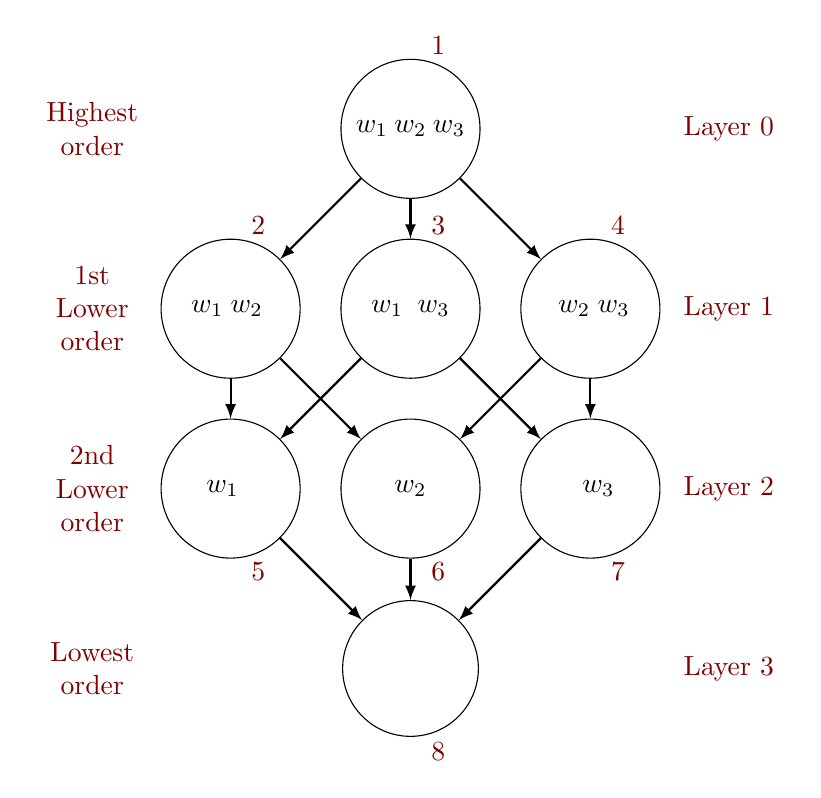
\begin{tikzpicture}
  \tikzset{
    state/.style  = {draw, circle, align = center, text centered, text width = 4.2em},
    invis/.style  = {text width = 4.2em},
    order/.style  = {align = center, text centered, text width = 4em, text = Maroon},
    number/.style = {xshift = 1em, text = Maroon},
  }

  \begin{scope}[node distance = 6.5em]
    \node [state] (000)                  {$w_1 \: w_2 \: w_3$};
    \node [invis] (000l) [left  of=000]  {};
    \node [invis] (000r) [right of=000]  {};

    \node [state] (001)  [below of=000l] {$w_1 \: w_2 \: \Skp$};
    \node [state] (010)  [below of=000]  {$w_1 \: \Skp \: w_3$};
    \node [state] (100)  [below of=000r] {$\Skp \: w_2 \: w_3$};

    \node [state] (011)  [below of=001] {$w_1 \: \Skp \: \Skp$};
    \node [state] (101)  [below of=010] {$\Skp \: w_2 \: \Skp$};
    \node [state] (110)  [below of=100] {$\Skp \: \Skp \: w_3$};

    \node [state] (111)  [below of=101] {$\Skp \: \Skp \: \Skp$};
    \node [invis] (111l) [below of=011] {};
    \node [invis] (111r) [below of=110] {};
  \end{scope}

  \begin{scope}[node distance = 5em]
    \node [order] [left of=000l]  {Highest order};
    \node [order] [left of=001]   {1st Lower order};
    \node [order] [left of=011]   {2nd Lower order};
    \node [order] [left of=111l]  {Lowest order};

    \node [order] [right of=000r] {Layer 0};
    \node [order] [right of=100]  {Layer 1};
    \node [order] [right of=110]  {Layer 2};
    \node [order] [right of=111r] {Layer 3};
  \end{scope}

  \begin{scope}[node distance = 3em]
    \node [number] [above of=000] {1};
    \node [number] [above of=001] {2};
    \node [number] [above of=010] {3};
    \node [number] [above of=100] {4};
    \node [number] [below of=011] {5};
    \node [number] [below of=101] {6};
    \node [number] [below of=110] {7};
    \node [number] [below of=111] {8};
  \end{scope}

  \path[->, >=latex, thick]
    (000) edge (001)
    (000) edge (010)
    (000) edge (100)

    (001) edge (011)
    (001) edge (101)
    (010) edge (011)
    (010) edge (110)
    (100) edge (101)
    (100) edge (110)

    (011) edge (111)
    (101) edge (111)
    (110) edge (111);
\end{tikzpicture}
\end{document}

  \caption{
    $\ProbGLM$ backoff graph of order 3 for history $h = w_1 w_2 w_3$.
  }
  \label{fig:history-glm}
\end{figure}


We also call a graph that represents the inter-dependencies of probabilities
during the calculation of $\ProbGLM{w}{h}$ the \emph{binomial diamond} of order
$n = \NGramLength{h}$, because of its diamond-like shape, and a number of
properties:

\begin{enumerate}
  \item \label{itm:num-layers} Unlike the case of Modified Kneser-Ney Smoothing
    there is no longer one clear way to define a total order of all the
    histories in the graph.
    Instead, if we partitioned the graph into layers, where layer $l$ contains
    the histories that have exactly $l$ skip words,
    the graph has $n + 1$ layers.
  \item \label{itm:num-childs} Layer $l$ contains exactly $\binom{n}{l}$ nodes.
  \item \label{itm:num-edges}  Nodes in layer $l$ have exactly $n - l$ outgoing
    and $l$ incoming edges.
  \item \label{itm:num-nodes}  There are $2^n$ nodes in the graph.
\end{enumerate}

\Cref{itm:num-layers} is due to the fact that layer $l$ includes exactly the
histories that are part of the $k$th highest order of probability.

To explain \cref{itm:num-childs}, it is helpful to imagine replacing words in
a history as laying a mask of either a skip or a non-skip on top of each word.
Then the number of nodes in each layer can be understood as permuting the
skip and non-skip masks on top of the history.
It is a well known fact that there are exactly $\binom{n}{l}$ permutations of
$l$ tokens of type A (skips) and $k$ tokens of type B (non-skips) when
$n = l + k$.

\Cref{itm:num-edges} directly follows from the fact that each non-skip word
in a history can be replaced by a skip, and that each skip is the result
of these replacements.

Last, we can explain \cref{itm:num-nodes} because every history is simply the
result of laying a mask which consists of a combination of skips or non-skips on
top of the original history.
All possible masks are therefore all permutations of two elements (skips or
non-skips) with repetition of length $n$, which there are $2^n$ arrangements of.
We can also infer this from \cref{itm:num-childs} via the binomial theorem
$(x+ y)^n = \sum_{l=0}^n \binom{n}{l} x^{n-l} y^l$, if we set ${x = y = 1}$,
we obtain $\sum_{k=0}^n \binom{n}{l} = 2^n$.

Following the model of the backoff graph will be a major aid in understanding
the weighted sum representation of the Generalized Language Model.

In order to have a notation available for all derived histories, we impose an
arbitrary total ordering on the histories.
One such ordering is given in \cref{fig:history-glm} and assigns each history
a number between $1$ and $8$.
Let $\DerivedHistory[i]$ than be the $i$th history of an arbitrary, but fixed
ordering.

% - - - - - - - - - - - - - - - - - - - - - - - - - - - - - - - - - - - - - - -
\subsection{Number of Sum Weights}

In the previous subsection, it was reasoned that, in the Generalized Language
Model, for a history of length $n$ there are exactly $2^n$ possible derivative
histories.
Following this, one might make the assumption, that to evaluate $\ProbGLM{w}{h}$
it is necessary to evaluate at most $2^n - 1$  different lower order
probabilities $\ProbGLM*{w}{\partial^* h}$ where $\partial^* h$ is any of the
$2^n - 1$ derived histories of $h$ excluding $h$ itself.
This assumption however is wrong as it can be necessary that, in the presence of
unseen histories, one history $\DerivedHistory[i]$ is both part of a highest
order probability $\ProbGLM{w}{\DerivedHistory[i]}$ and a lower order
probability $\ProbGLM*{w}{\DerivedHistory[i]}$, as will be shown in the next
paragraph.

\begin{subequations}
  Let us for example calculate the probability $\ProbGLM{w_3}{w_1 w_2}$ on
  hypothetical training data.
  That hypothetical training data shall be different from
  \cref{subsec:weightedsum-glm-example} and now $w_1 w_2$ shall be unseen,
  ergo $\Count(w_1 w_2) = 0$.
  Because of this, following \cref{eq:glm-backoff}, the average of backoff
  probabilities to be formed:
  \begin{equation}
    \ProbGLM{w_3}{w_1 w_2} = \frac{1}{2} \left( \ProbGLM{w_3}{\Skp w_2} + \ProbGLM{w_3}{w_1 \Skp}\right)
  \end{equation}
  Note that these backoff probabilities for histories $\Skp w_2$ and $w_1 \Skp$
  are still of the highest order $\ProbGLM$.
  We now further assume history $\Skp w_2$ to also not occur in training, so that
  further backoff is necessary.
  History $w_1 \Skp$ however is treated as seen:
  \begin{align}
    \label{eq:glm-example-unseen}
    \ProbGLM{w_3}{\Skp w_2} &= \ProbGLM{w_3}{\Skp \Skp} \\
    \label{eq:glm-example-seen}
    \ProbGLM{w_3}{w_1 \Skp} &= \frac{\Count(w_1 \Skp w_3) + \gamma(w_1 \Skp) \ProbGLM*{w_3}{\Skp \Skp}}
                                    {\Count(w_2 \Skp \Skp)}
  \end{align}
  We can see that $\ProbGLM{w_3}{\Skp \Skp}$ (\cref{eq:glm-example-unseen}) and
  $\ProbGLM*{w_3}{\Skp \Skp}$ (\cref{eq:glm-example-seen}) both factor into
  probability $\ProbGLM{w_3}{w_1 w_2}$.
  They would be evaluated as:
  \begin{align}
    \ProbGLM {w_3}{\Skp \Skp} &= \frac{\Count(\Skp \Skp w_3)}{\Count(\Skp \Skp \Skp)} \\
    \ProbGLM*{w_3}{\Skp \Skp} &= \frac{\ContCountIp(\WSkp \Skp \Skp w_3)}{\ContCountIp(\WSkp \Skp \Skp \WSkp)}
  \end{align}
\end{subequations}

Because of this, it is possible that one history $\DerivedHistory[\DummyIndex]$
might both occur as highest order probability
$\ProbGLM{w}{\DerivedHistory[\DummyIndex]}$ and lower order probability
$\ProbGLM*{w}{\DerivedHistory[\DummyIndex]}$.
It is non-trivial to decide exactly how many derived histories occur both as
highest and lower order probabilities, and to fit algorithms to this finding.
Consequently, we only employ an upper bound of sum weights $N$ and set all
unnecessary sum weights to zero.
An upper bound for the number of sum weights is the number of derived histories
times two, as histories can occur both in highest and lower order probabilities:
\begin{equation}
  \label{eq:weightedsum-glm-num}
  N = 2 \cdot 2^\NGramLength{h}
\end{equation}

% - - - - - - - - - - - - - - - - - - - - - - - - - - - - - - - - - - - - - - -
\subsection{Sum Terms}

Based on this we can define the sum terms for $1 \leq i \leq N$.
\begin{subequations}
  \begin{align}
    \label{eq:glmarg-high}
    \SumArg_{2 i - 1}^h(w) &=
      \begin{dcases*}
        \DiscountedCount(\DerivedHistory[i] w)        & if $\NumSkpOp{\DerivedHistory[i]} > 0$ \\
        \Count(\DerivedHistory[i] w)                  & if $\NumSkpOp{\DerivedHistory[i]} = 0$
      \end{dcases*} \\
    \label{eq:glmarg-low}
    \SumArg_{2 i}^h(w) &=
      \begin{dcases*}
        \DiscountedCount*(\WSkp \DerivedHistory[i] w) & if $\NumSkpOp{\DerivedHistory[i]} > 0$ \\
        \ContCountIp(\WSkp \DerivedHistory[i] w)      & if $\NumSkpOp{\DerivedHistory[i]} = 0$
      \end{dcases*}
  \end{align}
\end{subequations}
The terms with an odd index (\cref{eq:glmarg-high}) correspond to
$\DerivedHistory[i]$ occurring as the highest order of probability, the terms
with an even index (\cref{eq:glmarg-low}) to lower orders.
The case of $\NumSkpOp{\DerivedHistory[i]} = 0$ occurs when $\DerivedHistory[i]$
consists only of skips, it thus can no longer be backoffed, and therefore
presents the unigram case.

Finding the sum weights $\SumWeight^h_i$ is more complex.
We will first reason about how these weights have to be structured and then
give a more rigorous definition.
%We will first discuss weights for $\SumArg^h_{2 i - 1}(w)$, that is for the
%terms that compose the highest order.
The sum weights $\SumWeight^h_{2 i - 1}$, that are multiplied with
$\SumArg^h_{2 i - 1}(w)$ which compose the highest order weight, will be
discussed first.
Our solution is oriented along the backoff graph.
The weight of a history is exactly then zero, if no backoff step of
\cref{eq:glm-backoff} reaches that history.
This occurs if for that history's node all histories of immediate parent nodes
are seen.
Conversely, this means that the sum weights $\SumWeight^h_{2 i - 1}$ are proportional
to the number of paths from the root note to the current node, for which the
current node's history is seen but the histories of all others nodes in the
path are not.

What also has to be considered is that in \cref{eq:glm-backoff} we divide the
sum of all backoff probabilities by their count.
The more backoff steps that have to be performed to reach a node, the lower its
influence is.
However, in turn it also can be reached via more paths as seen in the backoff
graph of \cref{fig:history-glm}.
In total there exist two paths from the root node to any node in layer $2$.
But there exists a total of six paths from the root node to a node in layer
$3$.
We define a coefficient $\mu = \frac{(\NGramLength{h} - l_i)!}{\NGramLength{h}!}$,
where $l_i$ is the layer in the backoff graph in which the node of history
$\DerivedHistory[i]$ lies.
Sum weights $\SumWeight^h_i$ are also proportional to that coefficient $\mu$.

The final influence on $\SumWeight^h_{2 i - 1}$ stems from the fact that we
defined \cref{eq:glmarg-high} to only consist of the numerator of
\cref{eq:glm-high}.
Because of this we also have to divide the sum weight by the denominator of
that equation.

Sum weights $\SumWeight^h_{2 i}$ for terms that occur in lower orders are
calculated in an analogous way.
For the same argument as above they are also influenced by the coefficient
$\mu$ and a denominator, but this time that of \cref{eq:glm-low}.
However, for lower order weights they are also influenced by the denominators
of equations that included them.
This fact is especially visible by the nesting of fractions in
\cref{eq:probglmexpansion-inserted}.
From this equation we can conclude that a sum weight $\SumWeight^h_{2 i}$ of a
node is as sum of recursive calls from the root probability $\Prob{w}{h}$ to
the current node.
The chains of recursive calls that can reach a history $\DerivedHistory[i]$ are
exactly represented by the paths to it in the backoff graph.
Each node contributes a $\frac{\gamma}{\text{denominator}}$ weight.
Lower order sum weights thus consists of sums of multiplications, where the
factors are based on the nodes along a path to the current node.
\todo{Additional explanation of $factor \cdot sum$ property.}

Because of this complexity of terms that compose the sum weights, we will not
try to find a mathematical expression that defines these sum weights.
Instead, we will define them by specifying the algorithm that computes them:
Sum weights $\SumWeight^h_i$ are calculated by \cref{alg:weightedsum-glm} which
uses the auxiliary functions of \cref{alg:weightedsum-glm-helper}.

%\begin{algorithm}
%  \begin{algorithmic}[1]
%    \Function{calcCoefficient}{$level$, $order$}
%      \Rene[inline]{This is cached, right?}
%      \State $\mu = 1$
%      \For{$i \gets 1 \mathinner{\ldotp \ldotp} level$}
%        \State $\mu \gets \frac{\mu}{order - i + 1}$
%      \EndFor
%      \State \textbf{return} $\mu$
%    \EndFunction
%  \end{algorithmic}
%\end{algorithm}

\begin{algorithm}[t]
  \caption{Computing Generalized Language Model sum weights}
  \label{alg:weightedsum-glm}
  \begin{algorithmic}[1]
    \Require $h$
      \Comment{history for which to determinate sum weights}
    \Ensure $\SumWeight_1^h, \: \ldots, \: \SumWeight_N^h$
      \Comment{list of sum weights}

    %\State $n \gets \NGramLength{h}$
    %  \Comment{$n$-gram length of history $h$}
    \State $N \gets 2 \cdot 2^\NGramLength{h}$
      \Comment{number of sum factors}
      \label{ln:glm-numfactors}
    \For{\textbf{each} node \textbf{in} graph}
      \label{ln:glm-fornodesingraph}
      \LineComment{data lookup}
      \State node.count $\gets \Count(\DerivedHistory[\text{node.index}] \Skp)$
        \label{ln:glm-lookup-count}
      \State node.contCount $\gets \ContCountIp(\WSkp \DerivedHistory[\text{node.index}] \WSkp)$
        \label{ln:glm-lookup-contcount}
      \State node.gamma $\gets \gamma(\DerivedHistory[\text{node.index}])$
        \label{ln:glm-lookup-gamma}
      \State $\mu \gets \frac{(\NGramLength{h} - \text{node.layer})!}{\NGramLength{h}!}$
        \label{ln:glm-lookup-coeff}

      \vspace{1.0em}
      \LineComment{weight for highest order}
      \If{node.count $= 0$}
        \label{ln:glm-if-highweight-zero}
        \State $\SumWeight_{2 \cdot\, \text{node.index} - 1}^h \gets 0$
          \label{ln:glm-highweight-zero}
      \ElsIf{node $=$ root}
        \label{ln:glm-if-highweight-root}
        \State $\SumWeight_{2 \cdot\, \text{node.index} - 1}^h \gets \frac{1}{\text{node.count}}$
          \label{ln:glm-highweight-frac}
      \Else
        \label{ln:glm-if-highweight-else}
        \State $\SumWeight_{2 \cdot\, \text{node.index} - 1}^h \gets \dfrac{\mu \cdot \text{\Call{highestOrderWeight}{root, node}}}{\text{node.count}}$
          \label{ln:glm-highweight-rec}
      \EndIf

      \vspace{0.7em}
      \LineComment{weight for lower orders}
      \If{node.contCount $= 0$ \textbf{or} node $=$ root}
        \label{ln:glm-if-lowweight-zero}
        \State $\SumWeight_{2 \cdot\, \text{node.index}}^h \gets 0$
          \label{ln:glm-lowweight-zero}
      \Else
        \label{ln:glm-if-lowweight-else}
        \State $\SumWeight_{2 \cdot\, \text{node.index}}^h \gets \dfrac{\mu \cdot \text{\Call{lowerOrdersWeight}{root, node, \textbf{true}}}}{\text{node.contCount}}$
          \label{ln:glm-lowweight-rec}
      \EndIf
    \EndFor
    \algstore{glmbreak}
  \end{algorithmic}
\end{algorithm}

\begin{algorithm}[t]
  \caption{Auxiliary functions for GLM sum weight computation}
  \label{alg:weightedsum-glm-helper}
  \begin{algorithmic}[1]
    \algrestore{glmbreak}
    \Function{highestOrderWeight}{ancestor, node}
      \If{ancestor.count $\neq 0$}
        \label{ln:highhlp-count-nonzero}
        \Comment{if ancestor is seen}
        \State \textbf{return} $0$
          \Comment{this path does not contribute to highest order}
          \label{ln:highhlp-return-zero}
      \EndIf

      \vspace{0.7em}
      \If{ancestor.\Call{isParentOf}{node}}
        \label{ln:highhlp-isparent}
        \Comment{end of path?}
        \State \textbf{return} $1$
          \label{ln:highhlp-return-one}
      \EndIf

      \vspace{0.7em}
      \State sum $\gets 0$
        \label{ln:highhlp-init-sum}
      \For{\textbf{each} child \textbf{in} ancestor.\Call{childs}{$ $}}
        \label{ln:highhlp-for}
        \If{child.\Call{isAncestorOf}{node}}
          \label{ln:highhlp-isancestor}
          \State sum $\gets$ sum $+ {}$ \Call{highestOrderWeight}{child, node}
            \label{ln:highhlp-add}
        \EndIf
      \EndFor
      \State \textbf{return} sum
        \label{ln:highhlp-return}
    \EndFunction

    % --------------------------------------------------------------------------
    \vspace{0.7em}
    \Statex\hrule

    \Function{lowerOrdersWeight}{ancestor, node, firstSeen}
      \LineComment{calculate mult}
      \If{firstSeen \textbf{and} ancestor.count $\neq 0$}
        \label{ln:lowhlp-count-nonzero}
        \State factor $\gets \frac{\text{ancestor.gamma}}{\text{ancestor.count}}$
          \label{ln:lowhlp-from-highhlp}
        \State firstSeen $\gets$ \textbf{false}
          \label{ln:lowhlp-firstseen}
      \ElsIf{ancestor.contCount $\neq 0$}
        \label{ln:lowhlp-contcount-nonzero}
        \State factor $\gets \frac{\text{ancestor.gamma}}{\text{ancestor.contCount}}$
          \label{ln:lowhlp-from-lowhlp}
      \Else
        \label{ln:lowhlp-else}
        \State factor $\gets 1$
          \label{ln:lowhlp-one}
      \EndIf

      \vspace{0.7em}
      \If{ancestor.\Call{isParentOf}{node}}
        \label{ln:lowhlp-isparent}
        \Comment{end of path?}
        \If{firstSeen}
          \label{ln:lowhlp-isseen}
          \State \textbf{return} $0$
            \label{ln:lowhlp-return-zero}
            \Comment{node occurs as highest order for this path}
        \EndIf{}
        \State \textbf{return} mult
          \label{ln:lowhlp-return-mult}
      \EndIf

      \vspace{0.7em}
      \State sum $\gets 0$
        \label{ln:lowhlp-init-sum}
      \For{\textbf{each} child \textbf{in} ancestor.\Call{childs}{$ $}}
        \label{ln:lowhlp-for}
        \If{child.\Call{isAncestorOf}{node}}
          \label{ln:lowhlp-isancestor}
          \State sum $\gets$
            \label{ln:lowhlp-add-1}\\
            \hfill sum $+$ \Call{lowerOrdersWeight}{child, node, firstSeen}
            \label{ln:lowhlp-add-2}
        \EndIf{}
      \EndFor
      \State \textbf{return} factor $\cdot$ sum
        \label{ln:lowhlp-return}
    \EndFunction
  \end{algorithmic}
\end{algorithm}

The algorithm works with the notion of a backoff graph as shown in
\cref{fig:history-glm}.
That graph is unique for every history $h$ and consist of $2^\NGramLength{h}$
nodes.
Each node is assigned a derived history.
A directed edge from node $A$ to node $B$ is drawn if $B$'s history can be
created by replacing one word in $A$'s history with a skip $\Skp$.

\emph{Parents} of a node $A$ are all nodes $B$ that have a directed edge from
$B$ to $A$.
\emph{Children} of a node $A$ are all the nodes, that $A$ is a parent of.
\emph{Ancestors} of a node $A$ are all nodes that can be reached from $A$
by repeated application of the parent relation.
A \emph{path} exists to node $A_1$ from node $A_m$, if there is a set of nodes
$\Set{A_1, \ldots, A_m}$ such that it holds for all nodes $A_i$ in that set,
that $A_{i+1}$ is a parent of $A_i$ for $1 \leq i < m$.
The \emph{root} of a graph is the node that has no parents and is an ancestor
to all other nodes.
% The path to $A_1$ from $A_m$ then consists of all the nodes of that set.

To assign sum weights $\SumWeight^h_{2 i - 1}$ and $\SumWeight^h_{2 i}$ to
every history $\DerivedHistory[i]$ of the backoff graph we iterate over all
nodes in the graph in \cref{ln:glm-fornodesingraph}.
First some required data is prefetched
(\cref{ln:glm-lookup-count,ln:glm-lookup-contcount,ln:glm-lookup-gamma,ln:glm-lookup-coeff}),
then the highest order weight is computed
(\cref{ln:glm-if-highweight-zero,ln:glm-highweight-zero,ln:glm-if-highweight-root,ln:glm-highweight-frac,ln:glm-if-highweight-else,ln:glm-highweight-rec}),
and last that for lower orders
(\cref{ln:glm-if-lowweight-zero,ln:glm-lowweight-zero,ln:glm-if-lowweight-zero,ln:glm-if-lowweight-else,ln:glm-lowweight-rec}).

\emph{node.index} is simply the position of the total ordering of the backoff
graph the node got assigned.
The actual ordering does not matter, it however has to be consistent such that
$\DerivedHistory[\text{node.index}]$ is the history that belongs to that node.
Accessing a count value like $\Count(\DerivedHistory[\text{node.index}] \Skp)$
in \cref{ln:glm-lookup-count} is a potentially expensive operation, as a
separate data structure has to be queried.
\emph{node.count}, \emph{node.contCount}, and \emph{node.gamma} shall simply be
floating point variables that are stored local to each node and are thus quickly
accessible.
A possible implementation that supports this is showcased in
\cref{subsec:weightedsum-glm-implementation}.
\Cref{ln:glm-lookup-coeff} is listed under data lookup because the computation
of $\mu$ can simply be replaced by a lookup to a precomputed table with a
two-dimensional key. \emph{node.layer} is the layer of the node in the
backoff graph.

The properties \emph{node.count}, \emph{node.contCount}, and
\emph{node.gamma} are not only needed for calculations of the current node, but
also for the ones of all its descendants (for example
\cref{ln:highhlp-count-nonzero}).
Because of this an implementation has to ensure that the for-each loop in
\cref{ln:glm-fornodesingraph} only iterates over a node in layer $l$ if all
nodes of $l-1$ have been previously iterated.

Next the highest order weight $\SumWeight^h_{2 i - 1}$ is calculated.
That weight is zero if the node's history is unseen
(\cref{ln:glm-if-highweight-zero,ln:glm-highweight-zero}), as of
\cref{eq:glm-backoff}.
If the current node is the root node, we can specify the weight directly
(\cref{ln:glm-if-highweight-root,ln:glm-highweight-frac}), as of
\cref{eq:glm-high}.
Else we will have to apply the reasoning we outlined above and define the sum
weight as the fraction of coefficient $\mu$, number of paths, and denominator
(\cref{ln:glm-if-highweight-else,ln:glm-highweight-rec}).
\Call{highestOrderWeight}{\emph{ancestor}, \emph{node}} is a auxiliary function
that just counts the number of paths that only spans unseen nodes from
an \emph{ancestor} node to the current \emph{node} in a recursive manner.

Last, the weight $\SumWeight^h_{2 i}$ for lower orders is calculated.
Again if the term that would occur in the denominator \emph{node.contCount} is
zero, that term is assigned a weight of zero.
This also happens for the root note, as it can never occur in a lower order term
(\cref{ln:glm-if-lowweight-zero,ln:glm-lowweight-zero}).
Else a similar term to the highest order weight is computed, however with a
different auxiliary function
(\cref{ln:glm-if-lowweight-else,ln:glm-lowweight-rec}).

That auxiliary function \Call{lowerOrdersWeight}{\emph{ancestor}, \emph{node},
\emph{firstSeen}} forms the core of the algorithm.
We have reasoned above that the weight for lower orders is proportional to
a sum of multiplications, where each multiplication is built out of one path
from the root to the current node and each node contributes a
$\frac{\gamma}{\text{denominator}}$ factor.
This however depends on the node: if a node is the first seen one on the path
it contributes a
$\gamma(\DerivedHistory[\DummyIndex]) \div \Count(\DerivedHistory[\DummyIndex] \Skp)$
factor (\cref{ln:lowhlp-count-nonzero,ln:lowhlp-from-highhlp}) as of
\cref{eq:glm-high}. Following nodes on the path contribute a
$\gamma(\DerivedHistory[\DummyIndex]) \div \ContCount(\WSkp \DerivedHistory[\DummyIndex] \WSkp)$
factor (\cref{ln:lowhlp-contcount-nonzero,ln:lowhlp-from-lowhlp}) as of
\cref{eq:glm-low}.
Nodes that are unseen contribute the neutral element of multiplication, i.e.\
they don't change the weight (\cref{ln:lowhlp-else,ln:lowhlp-one}) as of
\cref{eq:glm-backoff}.

Also, we don't just compute sums of multiplications but instead apply
the distributive property were possible to reduce computational cost.
Each recursive step of the auxiliary function thus returns only a \emph{factor}
times \emph{sum} product, where the sum consists of incarnations of further
recursion depth
(\cref{ln:lowhlp-init-sum,ln:lowhlp-for,ln:lowhlp-isancestor,ln:lowhlp-add-1,ln:lowhlp-add-2,ln:lowhlp-return}).

% - - - - - - - - - - - - - - - - - - - - - - - - - - - - - - - - - - - - - - -
\subsection{Implementation}
\label{subsec:weightedsum-glm-implementation}

% \newlength{\oldtextfloatsep}
% \setlength{\oldtextfloatsep}{\textfloatsep}
% \setlength{\textfloatsep}{0em}

\begin{lstlisting}[
  label = {lst:backoff-graph-c},
  float,
  caption = {C data structures to implement the backoff graph},
  language = C,
]
  struct node {
    int count;
    int contCount;
    double gamma;
  };

  struct graph {
    char* history[n];
    struct node nodes[n * n]
  };
\end{lstlisting}

\begin{lstlisting}[
  label = {lst:next-in-order-index},
  float,
  caption = {C code to compute the next iteration index},
  language = C,
]
  if (index == 0)
      index = 1:
      return;

  int x = numberOfSetBits(index);

  // compute lexicographically next bit permutation
  // with x bits set
  int t = (index | (index - 1)) + 1;
  index = t | ((((t & -t) / (index & -index)) >> 1) - 1);

  // highest number with x bits set
  int m = ((1 << x) - 1) << (n - x);
  if (index > m)
      // next is smallest number with (x+1) bits
      index = (1 << (x + 1)) - 1;
  if (index > (1 << n) - 1)
      // restart, if next number would be more than n bits
      index = 0;
\end{lstlisting}

This subsection will explain our approach of implementing the backoff graph that
both consumes as little space as possible while being fast to traverse.
Our representation fits into a small contiguous amount of memory on the stack,
which will prevent cache misses, and thus result in access time improvements.

We reasoned in \cref{subsec:backoff-graph} that a backoff graph, for a history
$h$ with length $\NGramLength{h}$, has $2^\NGramLength{h}$ nodes.
Our core idea is now to store the graph into an array of $2^\NGramLength{h}$
\texttt{struct}s.

We will interpret each node's history as a binary number, where each set word
in the history becomes a zero and each skip becomes a one.
That is the node of history $w_1 \Skp w_3 w_4 \Skp$ for a graph of order $5$
is stored at the index $\texttt{01001}_2 = 9$.
That number is used as the index for each node in the array.
This representation makes it very fast to compute the layer, all parents, or
all children of a node.
These tasks can be specified entirely as bit operations, which should be
available as direct machine instructions for most architectures.
No materialized lists of all parents or all children are necessary.

The C code of \Cref{lst:backoff-graph-c} exhaustively lists necessary data
structures to implement \cref{alg:weightedsum-glm,alg:weightedsum-glm-helper}.
\texttt{n} has to be a predefined constant that specifies the (maximal) length
of histories.
The \texttt{struct} \texttt{node} consists of exactly the data members that are
used for data lookup storage in the algorithm.
\texttt{history} stores the $n$-gram $h$, and \texttt{nodes} bundles all nodes
of a graph in one instance.

We will now explain how all necessary data can be retrieved from that
representation:
\begin{itemize}
  \setlength{\itemsep}{0.4ex}
  \item The history $\DerivedHistory[i]$ of a node at index $i$ is simple
    the original \texttt{history}, where a skip $\Skp$ is placed at each
    position, where the node's index has a set bit.
  \item A node is the top root node if its index has no set bits, and in turn a
    node is the bottom leaf node if all bits in the index are set.
  \item The layer of a node is the number of set bits in its index.
  \item As explained in \cref{subsec:backoff-graph}, a node at layer $l$ has
    exactly $l$ parents and $\NGramLength{h} - l$ children.
  \item The index of the $i$th parent (child) of a node is found by unsetting
    (setting) the $i$th set (unset) bit.
  \item A node \texttt{A} is an ancestor of another node \texttt{B}
    if the bitwise and-operation on their indices returns \texttt{A}'s index
    respectively it is an descendant if the same holds for the bitwise or-
    operation:
    \begin{align*}
      \text{\texttt{A} ancestor of \texttt{B}} \: &\Leftrightarrow \: \texttt{A.index \& B.index == A.index} \\
      \text{\texttt{A} descendant of \texttt{B}} \: &\Leftrightarrow \: \texttt{A.index | B.index == B.index}
    \end{align*}
    with \texttt{\&} the bitwise-and, and \texttt{|} the bitwise-or.
\end{itemize}

The only non-trivial problem that follows from this representation is finding
the proper ordering of indices in which they should be accessed during an
in-order loop over the graph.
An in-order loop over the backoff graph iterates all nodes, such that a node
of layer $l$ is only accessed once all nodes of layer $l-1$ have been processed.

\Cref{lst:next-in-order-index} gives an algorithm in C code that generates the
next in-order index\footnote{The code to compute the lexicographically next bit
permutation is courtesy of
\mbox{\url{http://graphics.stanford.edu/~seander/bithacks.html\#NextBitPermutation}}
(accessed July 14, 2015).
It requires an architecture that stores negative integers in two's complement
format.}.
As input it requires the previous \texttt{index} and the backoff graph's order
$\texttt{n} = \NGramLength{h}$.
To ensure the fastest possible execution time the algorithm aims to be a minimal
composition of bit-level operations.

% \setlength{\textfloatsep}{\oldtextfloatsep}

% ------------------------------------------------------------------------------
\section{Monotonicity}
\label{sec:monotony}

We now want to prove that the probability definitions for Modified Kneser-Ney
Smoothing (\cref{sec:weightedsum-mkn}) and the Generalized Language Model
(\cref{sec:weightedsum-glm}) are monotonic functions on the $\SumArg^h_i(w)$.
This means that higher $\SumArg^h_i(w)$ values correspond to higher
probabilities.
We can formalize that property as:
\begin{equation}
  \big(\forall i \in \Set{1, \ldots, N}: \: \SumArg^h_i(w) \geq \SumArg^h_i(w^\prime)\big)
    \implies \Prob{w}{h} \geq \Prob{w^\prime}{h}
\end{equation}
This is an important property as it allows the application of top-$k$ joining
techniques in \cref{ch:topkjoin}.

Because we have defined these probabilities as sums of weights $\SumWeight^h_i$
multiplied with terms $\SumArg^h_i(w)$ (\cref{eq:weightedsum}), and since
addition and multiplication are trivially monotonic, it suffice to show that the
$\SumWeight^h_i$ are always non-negative to prove that our probability
definitions are monotonic.

To show that $\SumWeight^h_i$ are non-negative we take at look at their
definitions (\cref{eq:mkn-sumweight},
\cref{alg:weightedsum-glm,alg:weightedsum-glm-helper}),
and observe that they are defined as a combination (multiplication and
division) of occurrence counts $\Count(\DummyArg)$ and
$\ContCount_{1+}(\DummyArg)$, numbers of paths, and interpolation weights
$\gamma(\DummyArg)$.
Since by their nature occurrence counts and numbers of paths are natural
numbers, we only need to show that the interpolation weights
$\gamma(\DummyArg)$ are also non-negative.
These interpolation weights are defined as sums of discount values
$D_\DummyIndex$ multiplied with continuation counts
$\ContCount_\DummyIndex(\DummyArg)$ (\cref{eq:review-gamma}).
Since continuation counts again are defined as natural numbers, it remains to
prove that the discount values are non-negative.

A non-formal argument is the fact that the name and usage of discounting terms
would be nonsensical if negative values would be permitted.
Additionally we can derive this fact from the definition of the discounting
values $D_1, D_2, D_{3+}$ (\cref{eq:discounts}).
It is easy to see that these discounting values increase as the number of
n-grams $n_\DummyIndex$ in the corpus increases.
The factors $Y \frac{n_2}{n_1}$, $Y \frac{n_3}{n_2}$, $Y \frac{n_4}{n_3}$ reach
the limit of $\frac{1}{2}$ for an infinitely large corpus, and thus infinitely
large number of n-grams $n_\DummyIndex$.
As a result of the fact that these factors are limited, none of the discount
values can be negative.
Thereby we can see that our probability definitions are indeed monotonic.
